Below we consider 3- and 4-periodics in the confocal pair where $a,b$ are the semi-axes of the outer ellipse has axes $(a,b)$. Below, set $\delta=\sqrt{a^4-a^2 b^2+b^4}$ and $c^2=a^2-b^2$.

\subsection{N=3 case}

\begin{figure}
    \centering
    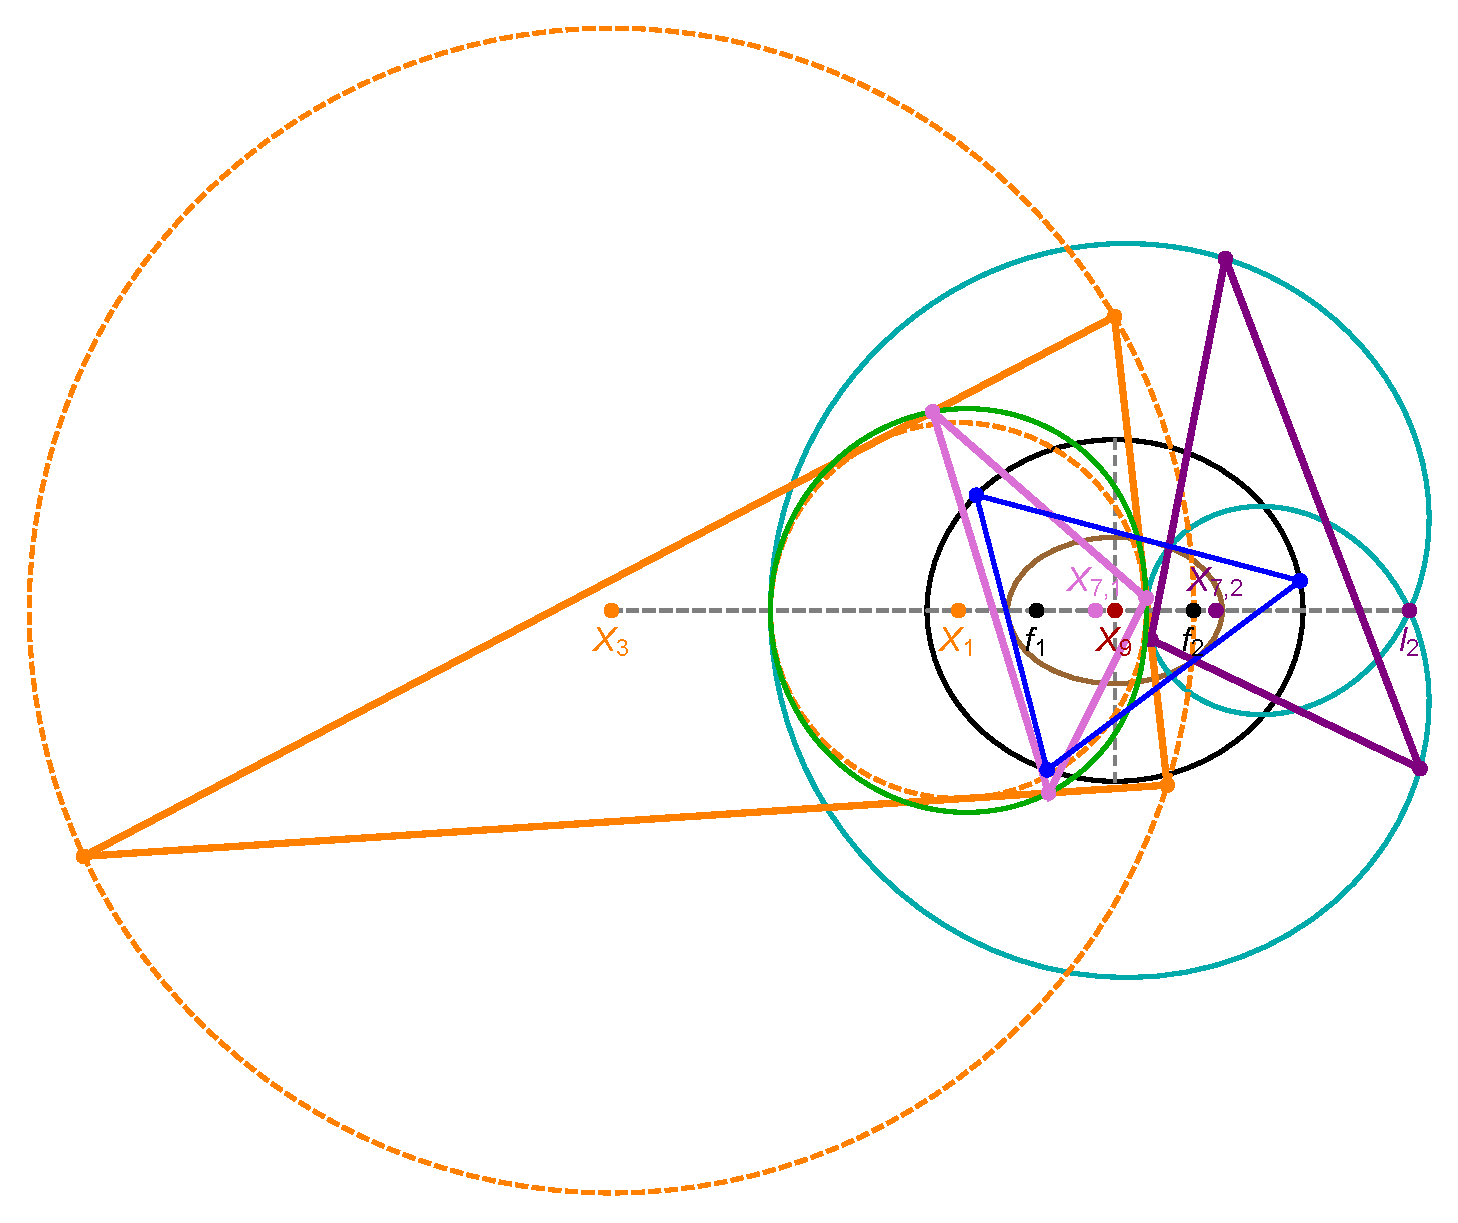
\includegraphics[width=.9\textwidth]{pics_05_0060_n3.pdf}
    \caption{N=3 case: the bicentric family (solid orange) is the poristic family \cite{gallatly1914-geometry}. Its sum of cosines is invariant and equal to those of the two limit point pedals (pink and purple). The Gergonne points $X_{7,1}$ and $X_{7,2}$ of each pedal are stationary. \href{https://bit.ly/379HU8l}{live}}
    \label{fig:n3}
\end{figure}

Referring to Figure~\ref{fig:n3}, the perimeter $L^\dagger$ of the inversive polygon for the $N=3$ family, originally derived in  \cite[Prop. 4]{reznik2020-n3-focus-inversive} is given by:


\[L^\dagger=L_+=\rho^2 \frac {\sqrt { \left( 8\,{a}^{4}+4\,{a}^{2}{b}^{2}+2\,{b}^{4}
 \right) \delta+8\,{a}^{6}+3\,{a}^{2}{b}^{4}+2\,{b}^{6}}}{{a}^{2}{b}^{
2}}\]

By Corollary~\ref{cor:inv-per}, this is equal to the perimeter $L_-$ of the bicentric pedal with respect to the focal limiting point.

\begin{align*}
    L_{-} &= {\frac {  \left( 9\,{R}^{2}-{d}^{2} \right)  \left( {R}^{2}-{d}^{2}
 \right) \sqrt {2}\rho^2}{16\,{R}^{4}d}\sqrt {- \left( {R}^{2}-{d}^{2}
 \right) ^{{\frac{3}{2}}}\sqrt {9\,{R}^{2}-{d}^{2}}+ 3R^4 + 6R^2d^2 - d^4}}\\
R&=(2a^4 - 2a^2b^2 + b^4 + (2a^2 -b^2)\delta  )a\rho^2/b^6,\;\;
d=(2a^2 - b^2 + 2\delta)c\rho^2a^2/b^6
\end{align*}

The perimeter $L_+$ of the bicentric pair with respect to the non-focal limiting point is given by:

\begin{align*}
    L_{+} &= {\frac { \left( 9\,{R}^{2}-{d}^{2} \right)  \left( {R}^{2}-{d}^{2}
 \right) \sqrt {2}\rho^2}{16\,{R}^{4}d}\sqrt { \left( {R}^{2}-{d}^{2}
 \right) ^{{\frac{3}{2}}}\sqrt {9\,{R}^{2}-{d}^{2}}+ 3R^4 + 6R^2d^2 - d^4}}\\
R&=(2a^4 - 2a^2b^2 + b^4 + (2a^2 -b^2)\delta  )a\rho^2/b^6,\;\;
d=(2a^2 - b^2 + 2\delta)c\rho^2a^2/b^6
\end{align*}

The sum of cosines of a triangle is given by $1+r/R$ and is therefore constant for the $N=3$ bicentric family. Let $\theta'_i$ denote the angles of the bicentric polygon. The sum  its cosines can be derived as:

\begin{equation}
\sum\cos\theta' = 1+\frac{r}{R} = \frac{3R^2 - d^2}{2R^2}
\label{eq:bic-cos}
\end{equation}

\begin{proposition}
The sum of cosines for the first and second $N=3$ bicentric pedals are constant and identical to \eqref{eq:bic-cos}.
\end{proposition}

Note: in terms of the associated elliptic billiard parameters, this is given by \cite[Prop. 6]{reznik2020-n3-focus-inversive}:

\[\sum\cos{\theta^\dagger}_{(N=3)}=\frac{\delta (a^2+c^2-\delta)}{a^2c^2} \]


\begin{proof} Using CAS, it follows from  straightforward calculations with the orbit parametrized in Appendix \ref{app:bicentric-vertices-n34}.
\end{proof}

The two limiting pedals have stationary Gergonne points $X_7$. The first one was derived in \cite[Proposition 1]{garcia2020-self-intersected}:

\[ X_{7,1}=\left[c\left(1-\frac{\rho^2}{\delta+c^2}\right),0\right]  \]


\[X_{7,1} =\frac{ (R^2 - d^2)((R^2 - d^2)^{3/2}\sqrt{9R^2 - d^2} + 3R^4 + 6R^2d^2 - d^4)}{16R^4d}\]

%\[X_{7,2}=-\frac{(R^2  -d^2) ((R^2 - %d^2)^{3/2}\sqrt{9R^2 - d^2} - 3R^4 - 6R^2d^2 + d^4)}{16d R^4}
%\]
\subsection{N=4 case}

\begin{figure}
    \centering
    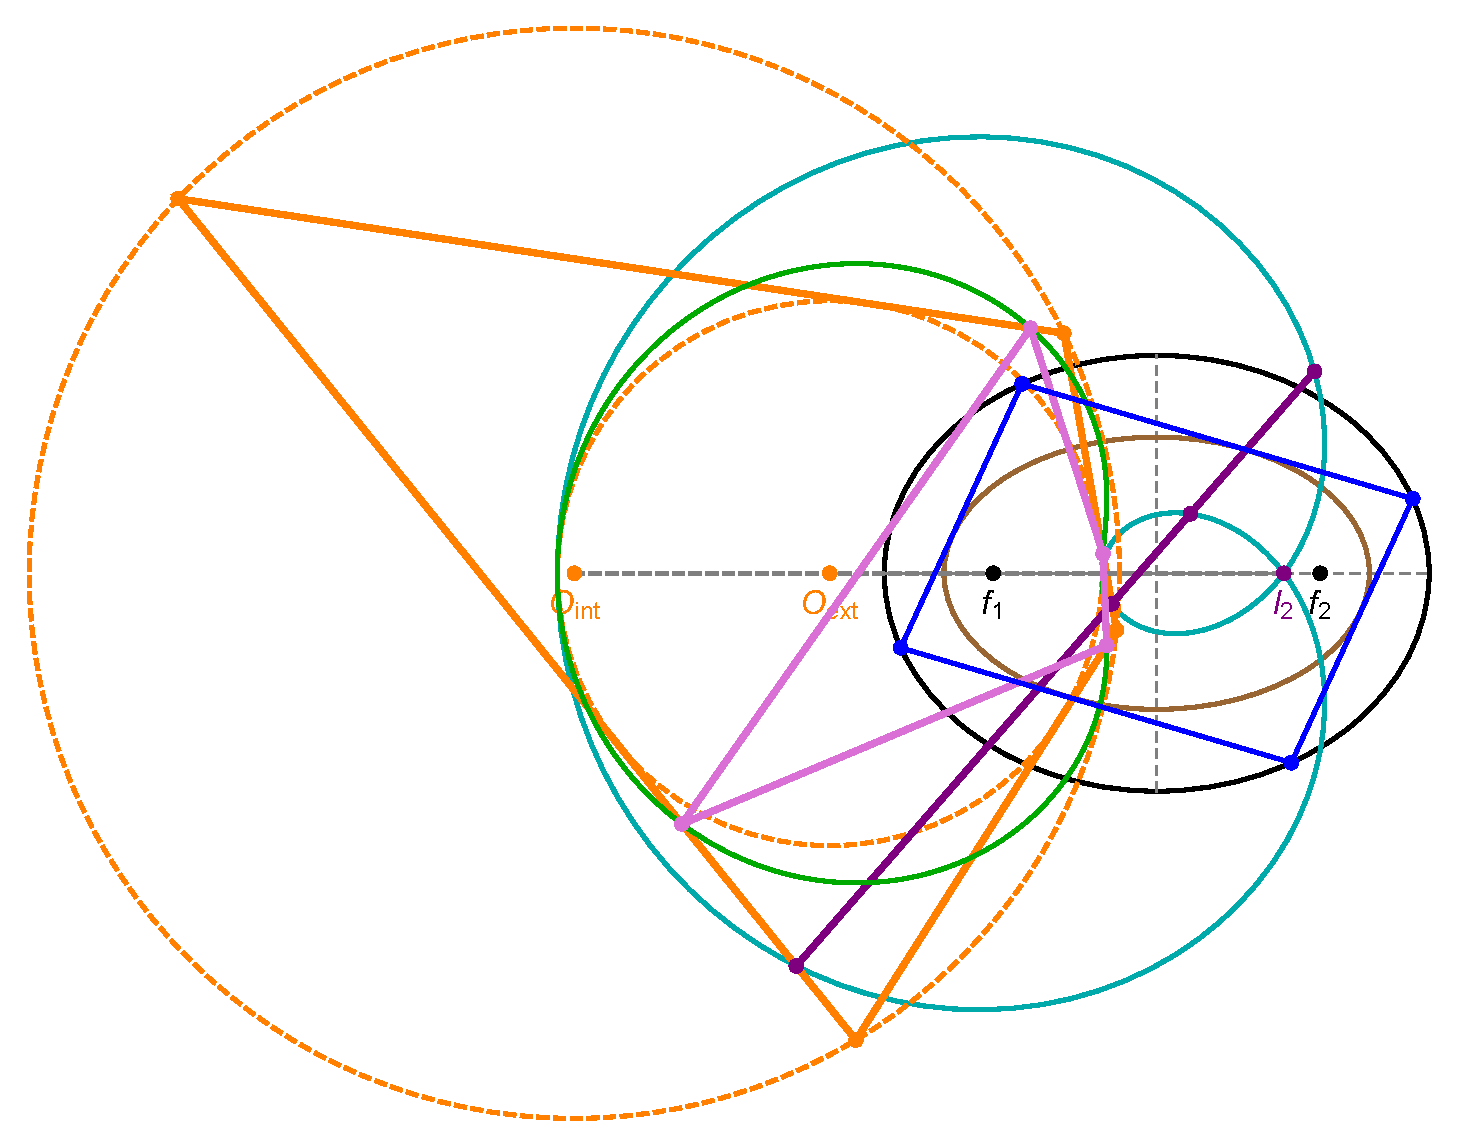
\includegraphics[width=.9\textwidth]{pics_05_0050_n4.pdf}
    \caption{In the N=4 case, remarkable things happen: (i) the sum of cosines of the $f_1$-pedal (pink) is not constant; (iii) its perimeter is the same as the corresponding billiard 4-periodic; (iv) the vertices of the $l_2$-pedal (purple) are collinear and (v) the sum of its cosines is 4. \href{https://youtu.be/fZe6elRTfeA}{Video}}
    \label{fig:n4}
\end{figure}

Referring to Figure~\ref{fig:n4}, the perimeter $L^\dagger$ of the inversive polygon for billiard 4-periodics was originally derived in  \cite[Prop. 18]{garcia2020-self-intersected}. It is identical to the perimeter of 4-periodics themselves and given by:

\begin{equation}
    L^\dagger= L_{+,N=4}= \,{\frac {4\sqrt {{a}^{2}+{b}^{2}}}{{b}^{2}}}
\label{eqn:inv-per-n4} 
\end{equation}

\begin{proposition}\label{prop:bicentricpedalN4}
In the $N=4$ family, the vertices of the bicentric pedal with respect to the non-focal limiting point are collinear.
\end{proposition}

\begin{proof}
The polar image of the bicentric family with respect to $\ell_2$ is a pair of confocal hyperbolas, see \cref{app:bicentric-to-confocal}, i.e., the polar image of bicentric 4-periodics is a billiard family. It can be shown its vertices are concyclic with the two hyperbolic foci $f_1',f_2'$, one of which coincides with $\ell_2$. Therefore, the inversion of said vertices with respect to $\ell_2$ is a set of collinear points.
\end{proof}

As before, Equation~\ref{eqn:inv-per-n4} is the same as the perimeter of the first bicentric pedal. The perimeter $L_+$ of the non-focal bicentric pedal is given by:

\[ L_{-,N=4} = \frac{4a^2}{b^2 c} \]

Regarding the sum of cosines, it is well-known a circle-inscribed quadrilateral has supplementary opposing angles, i.e.:

\begin{observation}
The sum of cosines of a bicentric N=4 family is null.
\end{observation}

Since the second bicentric pedal is a degenerate polygon:

\begin{observation}
The sum of cosines of the second limiting pedal to the N=4 bicentric family is equal to 4.
\end{observation}
